\documentclass{fict}

\addbibresource{references.bib}

\input{content/glossary}
\newacronym[description=Artificial intelligence]{ai}{AI}{Artificial Intelligence}
\newacronym[description=Computer Vision]{cv}{CV}{Computer Vision}
\newacronym[description=You only look once]{yolo}{YOLO}{You Only Look Once}
\newacronym[description=Segment anything model]{sam}{SAM}{Segment Anything Model}
\newacronym[description=Human pose estimation]{hpe}{HPE}{Human Pose Estimation}
\newacronym[description=Vision transformer]{vit}{ViT}{Vision Transformer}
\newacronym[description=Model-in-the-loop]{mitl}{MITL}{Model-in-the-Loop}
\newacronym[description=Convolutional neural network]{cnn}{CNN}{Convolutional Neural Network}
\newacronym[description=Region-based convolutional neural network]{rcnn}{R-CNN}{Region-based Convolutional Neural Network}
\newacronym[description=High-resolution network]{hrnet}{HRNet}{High-Resolution Network}
\newacronym[description=Non-maximum suppression]{nms}{NMS}{Non-Maximum Suppression}
\newacronym[description=Histogram of oriented gradients]{hog}{HOG}{Histogram of Oriented Gradients}
\newacronym[description=Scale-invariant feature transform]{sift}{SIFT}{Scale-Invariant Feature Transform}
\newacronym[description=Direct linear transformation]{dlt}{DLT}{Direct Linear Transformation}
\newacronym[description=Inertial measurement unit]{imu}{IMU}{Inertial Measurement Unit}
\newacronym[description=Interquartile range]{iqr}{IQR}{Interquartile Range}
\newacronym[description=Median absolute deviation]{mad}{MAD}{Median Absolute Deviation}
\newacronym[description=Mean average precision]{map}{mAP}{Mean Average Precision}
\newacronym[description=Mean absolute error]{mae}{MAE}{Mean Absolute Error}
\newacronym[description=Root mean square error]{rmse}{RMSE}{Root Mean Square Error}
\newacronym[description=Distribution focal loss]{dfl}{DFL}{Distribution Focal Loss}
\newacronym[description={Hue, saturation, value}]{hsv}{HSV}{Hue, Saturation, Value}
\newacronym[description=Graphics processing unit]{gpu}{GPU}{Graphics Processing Unit}
\newacronym[description=Neural processing unit]{npu}{NPU}{Neural Processing Unit}
\newacronym[description=Compute unified device architecture]{cuda}{CUDA}{Compute Unified Device Architecture}
\newacronym[description=Centre of mass]{com}{CoM}{Centre of Mass}
\newacronym[description=Common objects in context]{coco}{COCO}{Common Objects in Context}
\newacronym[description=Not a number]{nan}{NaN}{Not a Number}
\newacronym[description=The latest version of the YOLO-family of object detectors]{yolo26}{YOLO26}{YOLO26}

\title{AI-Based Stroke Phase Detection and Symmetry Analysis in Competitive Swimming Footage: A Proof of Concept}
\author{Daniel Pace}
\supervisor{Dr.\ Vanessa Camilleri}
% If you have no co-supervisor, remove the below line
% \cosupervisor{Dr Name Surname}
\degreename{Bachelor of Science in Information Technology (Honours) (Artificial Intelligence)}
\titledate{\today}

\begin{document}

\frontmatter{}
\pagestyle{pageNumbersOnly}

\input{content/title.tex}
\chapter*{Abstract}
\addcontentsline{toc}{chapter}{Abstract}

Computer vision analysis in aquatic environments presents unique challenges due to light refraction, surface turbulence, and occlusion, which hinder the accuracy of standard motion tracking systems. This project presents a non-intrusive, AI-based proof-of-concept system for extracting swimming kinematics from uncalibrated, handheld poolside video footage. The core contribution is a novel methodology for dynamic pixel-to-meter scaling using custom 3D-printed underwater markers as calibration objects, addressing the limitations of fixed-camera setups across varying pool environments. A Model-in-the-Loop annotation pipeline, combining SAM 2 temporal segmentation with statistical outlier filtering and human verification, was developed to construct a domain-specific training dataset for a fine-tuned YOLO26 marker detector. Ego-motion compensation, ViTPose-based hip localisation, and Kalman filter smoothing were combined to produce absolute positional and velocity profiles from raw tracking output. Evaluation on a 50 m breaststroke sequence yielded a mean absolute split-time error of 1.005 s and an RMSE of 1.210 s across 18 checkpoints, demonstrating the feasibility of metric-accurate swimmer tracking without specialised hardware. Wrist keypoint tracking remained noisy in the underwater environment, highlighting distal pose estimation as the primary target for future refinement.
\chapter*{Acknowledgements}
\addcontentsline{toc}{chapter}{Acknowledgements}

Completing this project has been simultaneously one of the most humbling and rewarding experiences of my life, and it wouldn't have been possible without those who supported me along the way.

Much like a swimming coach, Dr.\ Vanessa Camilleri, you have been a guiding force throughout this project, providing me with the tools, feedback, and encouragement I needed to navigate the turbulent waters of research. I am deeply grateful for your mentorship, patience, and belief in my abilities, which have been integral to my growth as a researcher and success in this project.

Just as the water holds up a swimmer, my family has been my support system. Keeping me afloat during the long hours of work and study, your love and encouragement have been the lifeline that kept me going.

Similar to how the lanerope stays by a swimmer's side, my friends and peers have been consistently present throughout this journey, providing companionship, distractions, and much-needed breaks that kept me sane. The moments we've shared will always be cherished, and I am grateful for the laughter and support that helped me through the challenges of this project.

As a swimming rival pushes one to improve themselves, I would like to thank my lecturers for inspiring the curiosity and thirst for learning that drove me to pursue this project in the first place. Your dedication to teaching and research has been a constant source of motivation, and I am grateful for the education and opportunities you have provided me. % should i change this to swimming clubmates?

Finally, as I've run out of swimming metaphors, I would like to address the swimming community, whose dedication and love for the sport genuinely inspire me to push my own boundaries. Thank you for showing me what passion and commitment looks like, and what never giving up really means.

\clearpage{}

\tableofcontents{}
\addcontentsline{toc}{chapter}{Contents}
\clearpage{}

\listoffigures{}
\addcontentsline{toc}{chapter}{List of Figures}
\clearpage{}

\listoftables{}
\addcontentsline{toc}{chapter}{List of Tables}
\clearpage{}

\printglossary[type=\acronymtype,nonumberlist,title=List of Abbreviations]
\addcontentsline{toc}{chapter}{List of Abbreviations}
\clearpage{}

\printglossary[nonumberlist,title=Glossary of Symbols]
\addcontentsline{toc}{chapter}{Glossary of Symbols}
\clearpage{}

\mainmatter{}
\pagestyle{MainMatter}

\chapter{Introduction}%
\label{chp:introduction}
The application of Artificial Intelligence (AI) and computer vision in the field of sports science has grown significantly, offering new avenues for performance analysis beyond traditional, subjective coaching methods. This Final Year Project (FYP) introduces a proof-of-concept system designed to leverage these technologies for the biomechanical analysis of competitive swimming. The system aims to provide objective, data-driven insights by detecting key stroke phases and quantifying limb symmetry in freestyle swimming footage.

The primary goals of this project are twofold: firstly, to develop a robust method for segmenting freestyle swimming motion into biomechanically relevant phases, such as the catch, pull, push, and recovery. Secondly, the project aims to establish a methodology for analyzing and quantifying the bilateral symmetry of a swimmer's limb movements. The approach used will involve applying an off-the-shelf pose estimation model to extract keypoint data from video footage. This keypoint sequence will then be processed using machine learning techniques to achieve the aforementioned goals.

A core assumption of this project is that existing datasets of swimming footage, such as those from the DIVE and SWIM-360 projects, can be used for initial development and testing. Furthermore, as a proof-of-concept, the system's final evaluation will be primarily qualitative, relying on annotated samples and feedback from experienced swimming coaches.

At a high level, the system will intake raw swimming video footage. It will then apply a pre-trained pose estimation model to identify and track the coordinates of a swimmer’s body joints. These keypoint data will form the basis for two subsequent analyses: a sequence modeling approach for stroke phase detection, and a comparative analysis of left and right limb trajectories to quantify symmetry. The final output will be a visual overlay on the video, providing immediate feedback on stroke phases and symmetry metrics.

This report is structured as follows: Chapter 1 introduces the project's context, aims, and methodology. Chapter 2 provides the necessary background information and a review of relevant literature. Chapter 3 details the system's design and architecture. Chapter 4 explains the implementation process. Chapter 5 presents the evaluation and testing of the prototype. Finally, Chapter 6 discusses future work and concludes the report.
\graphicspath{{content/chapters/2_background/figures/}}

\chapter{Background}%
\label{chp:background}

Existing literature in sports biomechanics highlights the importance of kinematic metrics like stroke length and propulsion symmetry. Computer vision research has successfully applied deep learning for human pose estimation (HPE) and action recognition in water sports. However, a critical limitation in many CV-based swimming systems is the inability to convert pixel movement into absolute, real-world distances, often relying on relative metrics or requiring external sensors.

This project draws upon two key areas of research:
\begin{itemize}
    \item \textbf{Scale Estimation}: Research on using planar objects or known reference markers (fiducial markers) for depth and scale estimation is relevant, which we adapt by using the structured, repetitive nature of the lanerope.
    \item \textbf{Kinematic Segmentation and Symmetry}: Work on segmenting continuous athletic motion (like running or swimming) into discrete phases is essential for calculating time-based metrics (e.g., wall contact time) and assessing symmetry by comparing left and right limb kinematic profiles.
\end{itemize}

\section{Proposed Solution: System Overview}
The proposed system is partitioned into three functional steps: Lanerope Calibration, Feature Extraction, and System Output.

\subsection{Step 1: Lanerope Calibration (Validation Reference)}
This step is the foundation of the system, establishing a stable axis and scale for all downstream measurements. It involves a comparative study of two approaches:
\begin{enumerate}
    \item \textbf{Traditional CV Pipeline}: Utilising colour thresholding (to isolate the coloured floats), edge detection (e.g., Canny), and Hough Transform or RANSAC for line fitting to project a stable reference line along the lanerope's center.
    \item \textbf{CNN-based Pipeline}: Implementing a keypoint detection or semantic segmentation model (e.g., a customised U-Net or Mask R-CNN) to identify the boundary or center points of the lanerope floats. This is expected to offer better robustness against water splash and varying lighting.
\end{enumerate}
The results of these two pipelines will be used to create the Calibration Module, converting pixel-based distances into real-world meters.

\subsection{Step 2: Feature Extraction – Starts, Swim, and Turns}
With the metric scale in place, a robust pose-estimation model will track the swimmer's key joints. A sequence-modelling approach will then segment the footage to extract biomechanical features across the three domains:
\begin{itemize}
    \item \textbf{Starts}: Metrics include reaction time, leap and flight times, underwater speed and distance, and shoulder/arm position at the end of the first pull.
    \item \textbf{Swim (Mid-Pool)}: Focus on stroke length (hand entry to exit in meters) and impulse (distance covered per stroke). This step will also facilitate the left–right symmetry assessment by comparing the angular and linear velocities of the corresponding limbs during the catch and pull phases.
    \item \textbf{Turns}: Metrics include stroke rate before the wall, entry-to-wall contact time, wall contact duration, and push-to-breakout measures (underwater distance and shoulder/arm positions leading to the second stroke).
\end{itemize}

\section{Evaluation Plan}
The evaluation strategy is two-fold, encompassing a rigorous quantitative assessment of the core technology and a qualitative validation of the final derived metrics.

\subsection{Quantitative Evaluation}
\begin{itemize}
    \item \textbf{Lanerope Accuracy Comparison}: The two lanerope pipelines (Traditional CV and CNN) will be assessed against annotated ground truth. Metrics will include axis error (deviation from the true lanerope angle), scale error (difference from the known float interval distance), and frame-to-frame jitter (stability).
    \item \textbf{Downstream Metric Accuracy}: The lanerope method yielding the lowest error will be used to calibrate the system. The final system's metric outputs (e.g., a calculated 5-meter distance) will be compared to a physically measured distance to quantify the final distance estimation accuracy.
\end{itemize}

\subsection{Qualitative Validation}
\begin{itemize}
    \item \textbf{Annotated Footage Comparison}: System outputs (keypoints, trajectories, and phase segmentations) will be overlaid onto the original video and validated against human-annotated samples.
    \item \textbf{Expert Feedback}: Structured interviews and feedback sessions will be conducted with certified swimming coaches to assess the interpretability, practical value, and actionability of the generated performance reports (e.g., symmetry score, wall contact duration).
\end{itemize}

\section{Conclusions including Expected Outcomes and Difficulties/Challenges}
This project is expected to deliver a robust proof-of-concept system capable of providing high-value, objective biomechanical data from standard video. The expected outcomes include the validated optimal lanerope calibration method (Traditional CV or CNN) and a working pipeline that accurately calculates and visualises metrics across Starts, Swim, and Turns.

Key challenges and difficulties anticipated include:
\begin{itemize}
    \item \textbf{Data Annotation}: Obtaining sufficient, high-quality, frame-by-frame annotated footage for training the CNN-based lanerope model and for ground-truthing the pose/phase segmentation.
    \item \textbf{Generalisation}: Ensuring the lanerope calibration method is robust against varying pool environments, lighting conditions, and camera angles (beyond a fixed setup).
    \item \textbf{Symmetry Complexity}: Developing a sufficiently sensitive metric to accurately quantify left–right symmetry, given the inherent small variances in human movement.
\end{itemize}

% % Figure~\ref{fig:sample} shows a sample figure and how to cross-reference
% % figures.
% %
% % \begin{figure}[htbp]
% %     \centering
% %     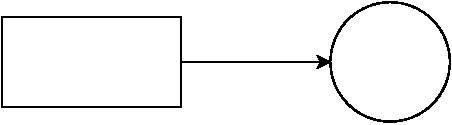
\includegraphics[width=\textwidth,keepaspectratio]{sample}
% %     \caption[Short sample caption.]{Longer caption that  and shows below the figure.\label{fig:sample}}
% % \end{figure}
% %


% \section{Literature Review}%
% \label{sec:literature_review}
% The effective analysis of swimming technique is a complex and crucial aspect of competitive swimming. Traditionally, this process has been performed by coaches who rely on their expertise and visual observation, often supplemented by slow-motion video playback. However, this manual approach is inherently subjective, time-consuming, and may miss subtle biomechanical inefficiencies. The emergence of AI and computer vision offers the potential to provide a more objective and consistent analysis, enabling swimmers and coaches to gain deeper insights into performance.

% This project's wider context is the burgeoning field of sports analytics, where AI is used to optimize training, prevent injuries, and enhance athletic performance across various disciplines. The anticipated benefits of the proposed system include the ability to provide instant, precise feedback on technique, helping swimmers to correct asymmetries and refine their stroke patterns. The likely users of this system are competitive swimmers, their coaches, and sports scientists seeking to research human motion.

% The theoretical foundation of this project lies in the fields of computer vision and machine learning. Specifically, the system will utilize pose estimation, a computer vision task that identifies the location of a person's joints from an image or video. This data is then used in a sequence modeling context to analyze temporal patterns of motion. The software development will utilize a programming language like Python, leveraging common AI libraries such as TensorFlow or PyTorch, and a chosen off-the-shelf pose estimation model.
% \section{Instructions}%
% \label{sec:instructions}

% This sentence refers to Section~\ref{sec:literature_review}, as an example of
% how to do cross-referencing.
% Equation~\eqref{eq:emc} shows one of the most famous equations.
% %
% \begin{equation}
%     \label{eq:emc}
%     e = mc^2
% \end{equation}
% %
% An example of how to create multiple equations, where they all align is given
% below.
% %
% \begin{align}
%     e & = mc^2          \\
%     m & = \frac{e}{c^2}
% \end{align}

% \section{Inserting references}%
% \label{sec:inserting_references}

% To insert a reference, the entry must be inserted in the \texttt{references.bib}
% file.
% The key or unique ID of the entry is then used to refer to it.
% \LaTeX{} will automatically number the entry and generate the list of
% references.
% The paper in~\cite{sample_key} is used as a referencing example.

% \section{Inserting acronyms}%
% \label{sec:inserting_acronyms_and_glossary_entries}

% The \gls{tcp} and \gls{udp} protocols are two layer 4 protocols, used for
% demonstrating how to use acronyms.
% On the second use of an acronym, only its initials are shown as demonstrated in
% the following sentence.
% The \gls{tcp} and \gls{udp} protocols are two layer 4 protocols, used for
% demonstrating how to use acronyms.

% \section{Using glossary terms}%
% \label{sec:using_glossary_terms}

% Let \gls{G} represent a loop-free directed graph, where \gls{V} and \gls{E}
% represent the set of nodes and edges, respectively.

% \section{Inserting a table}%
% \label{sec:inserting_a_table}

% A simple table is shown in Table~\ref{tab:simple}, with a more complex example
% given in Table~\ref{tab:complex}.

% \begin{table}
%     \caption{Simple table example.\label{tab:simple}}
%     \centering
%     \begin{tblr}{|c|S[table-format=3.2]|c|}
%         \hline
%         \textbf{Header 1} & \textbf{Header 2} & \textbf{Header 3} \\
%         \hline
%         1                 & 2.3               & Orange            \\
%         2                 & 100.5             & Blue              \\
%         3                 & 35.0              & Black             \\
%         \hline
%     \end{tblr}
% \end{table}

% \begin{table}
%     \centering
%     \caption{Complex table example.\label{tab:complex}}
%     \begin{tblr}{|Q[m,0.2\textwidth]|Q[m,0.2\textwidth]|Q[m,0.2\textwidth]|Q[m,0.2\textwidth]|}
%         \hline
%         \SetCell[r=2]{c} Table Head & \SetCell[c=3]{c} Table Column Head & & \\
%         \hline
%         & Table column subhead 1 & Table column subhead 2 & Table column subhead 3 \\
%         \hline
%         Item 1 & 2 & 3 & 4 \\
%         \hline
%         Item 2 & 2 & 3 & 4 \\
%         \hline
%         Item 3 & 2 & 3 & 4 \\
%         \hline
%         Item 4 & 2 & 3 & 4 \\
%         \hline
%     \end{tblr}
% \end{table}

% \section{Inserting code snippet}%
% \label{sec:inserting_code_snippet}

% The code snippet in Listing~\ref{lst:python_example} demonstrates a very simple
% python program.

% \begin{lstlisting}[language=Python,caption=Python example,label={lst:python_example}]
% def main() -> None:
%     print("Hello World")

% if __name__ == "__main__":
%     main()
% \end{lstlisting}

% \section{Inserting theorems, corollaries and lemmas}%
% \label{sec:inserting_theorems,_corollaries_and_lemmas}

% \begin{theorem}
%     Let \(f\) be a function whose derivative exists in every point, then \(f\) is
%     a continuous function.
% \end{theorem}

% \begin{theorem}[Pythagorean theorem]
%     \label{pythagorean}
%     This is a theorem about right triangles and can be summarised in the next
%     equation
%     \[ x^2 + y^2 = z^2 \]
% \end{theorem}

% And a consequence of theorem \ref{pythagorean} is the statement in the next
% corollary.

% \begin{corollary}
%     There's no right rectangle whose sides measure 3cm, 4cm, and 6cm.
% \end{corollary}

% You can reference theorems such as \ref{pythagorean} when a label is assigned.

% \begin{lemma}
%     Given two line segments whose lengths are \(a\) and \(b\) respectively there is a
%     real number \(r\) such that \(b=ra\).
% \end{lemma}

% \section{Inserting an algorithm}%
% \label{sec:inserting_an_algorithm}

% The pseudocode for a basic \gls{ea} using NSGA-II is given in
% Algorithm~\ref{alg:evolutionaryAlgorithm}.

% \begin{algorithm}
%     \caption{Pseudocode for an Evolutionary Algorithm}%
%     \label{alg:evolutionaryAlgorithm}
%     \begin{algorithmic}
%         \State \( \mathcal{P} \) = Population Size
%         \State \( \chi \) = Number of Generations
%         \State \( \omega \) = Crossover Probability
%         \State \( \psi \) = Mutation Probability
%         \State
%         \State population = GenerateInitialPopulation(\( \mathcal{P} \))
%         \For{\( 1, 2, \ldots, \chi \)}
%         \State offspring = TournamentSelection(population, \( \mathcal{P} \))
%         % Crossover
%         \For{\(c_i \in \) offspring, \( i = 1, 3, 5, \ldots, \mathcal{P}\)}
%         \State \(z\) = random(0, 1)
%         \If{\( z < \omega \)}
%         \State Crossover(\( c_i, c_{i+1} \))
%         \EndIf
%         \EndFor
%         % Mutation
%         \For{\(c_i \in \) offspring}
%         \State \(z\) = random(0, 1)
%         \If{\( z < \psi \)}
%         \State Mutate(\( c_i \))
%         \EndIf
%         \EndFor
%         % Calculate fitness
%         \State CalculatePopulationFitness(offspring)
%         % Update population size
%         \State population = NSGA-II([population + offspring], \(\mathcal{P}\))
%         \EndFor
%     \end{algorithmic}
% \end{algorithm}

\chapter{Literature Review}%
\label{chp:literature_review}

\section{Evolution of AI in Sports Analytics}
Computer vision (CV) has fundamentally altered the landscape of sports analytics, transitioning
from manual annotation to automated, high-fidelity measurement. Tracing the historical arc of
this evolution reveals a trajectory that began in the 1990s and early 2000s with manual
notational analysis. During this era, practitioners relied on painstaking frame-by-frame video
review and manual timing systems to derive basic performance metrics. The subsequent era of
``hand-crafted'' features saw the introduction of algorithms such as the Histogram of Oriented
Gradients (HOG), Scale-Invariant Feature Transform (SIFT), and various optical flow techniques.
While these early systems represented a step toward automation, they relied on heuristic-based
observation and were notoriously fragile, frequently failing under the non-uniform lighting and
high-entropy background noise characteristic of aquatic environments.

The paradigm shift occurred following the ``Deep Learning revolution,'' catalysed in large part
by the success of AlexNet in the 2012 ImageNet challenge~\cite{krizhevsky2012imagenet}. This
milestone demonstrated that hierarchical feature extraction through Deep Convolutional Neural
Networks (CNNs) could outperform any human-engineered descriptor. Building on the foundations
laid by earlier architectures such as LeNet~\cite{lecun2002gradient}, researchers began applying
deep learning to sports-specific tasks. In the mid-2010s, models such as
ResNet~\cite{he2016deep} became standard for robust feature representation, allowing for more
stable tracking in dynamic environments.

However, the adoption of these technologies has been uneven across the sporting landscape. Field
sports such as football, tennis, and athletics have received a disproportionate share of research
attention due to the relative ease of data collection in well-lit, terrestrial environments. In
contrast, swimming has lagged behind, primarily due to the unique optical challenges of the pool.
As noted by~\cite{Zhou2025}, AI-driven systems are now the standard for extracting kinematic
data and estimating pose in real time, but their application in swimming remains a frontier of
computer vision. The current paradigm is moving toward Foundation Models, defined as large-scale
models trained on massive, diverse datasets that exhibit zero-shot
generalisation~\cite{dosovitskiy2020image}. This thesis utilises models such as SAM~2 and
ViTPose, which provide a level of geometric and spatial reasoning, as well as temporal
consistency, previously unavailable in sports-specific contexts. Tools such as
DeepLabCut~\cite{mathis2018deeplabcut} and OpenPose~\cite{cao2019openpose} pioneered the
transfer of these capabilities to biomechanics, but the transition to the aquatic domain requires
a fundamental reassessment of how models perceive motion through water.

\section{An Adversarial Domain for Computer Vision}
While field sports such as football or athletics provide relatively stable visual environments
with predictable occlusions, the aquatic setting serves as an adversarial domain that
stress-tests the limits of image processing. Unlike terrestrial pose estimation, where the
medium of air is the standard, the water-air interface introduces non-linear geometric
distortions that violate the fundamental pinhole camera model
assumptions~\cite{agrawal2012theory}.

To understand the severity of this challenge, one must consider Snell's Law, which dictates that
$n_1 \sin \theta_1 = n_2 \sin \theta_2$. Because the refractive index of water ($n \approx
1.33$) differs significantly from air ($n \approx 1.00$), the apparent position of a swimmer's
joint underwater is displaced from its true anatomical
coordinate~\cite{harvey1998calibration}. Underwater camera systems require careful calibration
to compensate for this distortion, often necessitating specialised refractive camera models or
dedicated underwater calibration rigs~\cite{shortis2015calibration}. Without such compensation,
standard pose estimation models produce systematic errors in joint angle calculations, rendering
them insufficient for high-performance biomechanical analysis.

Beyond refraction, the environment is plagued by dynamic noise. As~\cite{giulietti_swimmernet_2023}
highlights, measurements are strongly influenced by disruptive elements such as bubbles, splashes,
and surface glare. These elements introduce severe, transient occlusions and
``caustics'', the dancing light patterns on the pool floor caused by the focusing effect of
surface waves. Indoor pool lighting often exacerbates these effects, creating high-contrast
reflections that can be mistaken for anatomical features by naive detectors. Furthermore,
swimming involves a unique ``multi-phase'' appearance problem: an athlete alternates between
above-water and below-water states. During a butterfly stroke recovery or a freestyle tumble
turn, the swimmer's body undergoes sudden, drastic changes in visual texture and limb visibility
that have no direct terrestrial analogue.

These environmental stressors explain why terrestrial benchmarks, such as
COCO~\cite{lin2014microsoft} or the MPII Human Pose dataset~\cite{andriluka20142d}, are largely
inadequate for the aquatic domain. While a model trained on COCO may excel at identifying a
pedestrian on a sidewalk, it lacks exposure to the blurred, refracted, and partially occluded
silhouettes of a submerged athlete. Einfalt et al.~\cite{einfalt2018activity} demonstrate that
even fine-tuned CNNs evaluated on real swimming footage exhibit systematic error modes in the
aquatic environment, confirming that models pre-trained on terrestrial data generalise poorly to
this domain. This necessitates the use of temporal memory mechanisms, such as the memory bank
implemented in SAM~2~\cite{ravi2024sam}, which allows a system to maintain object features even
when they are obscured by a splash or submerged beyond clear visibility. By treating the aquatic
environment as a structured noise problem rather than random interference, temporal dependencies
can be exploited to maintain tracking where classical optical flow methods fail systematically.

\section{From Handcrafted Features to Foundation Models}
Historically, structural feature detection in swimming relied on the Hough Transform or
colour-keying to isolate lane ropes or markers. However, these methods break down under varying
pool illumination and water turbulence~\cite{holzmann_measuring_2012}. Colour-keying, for
instance, is highly susceptible to the ``blue-shift'' of underwater light, whereby longer
wavelengths are absorbed more rapidly, causing markers to lose their distinct chromatic
signatures at depth. Similarly, classical optical flow algorithms such as Lucas-Kanade fail in
the presence of ``aperture problems'' caused by the repetitive, textureless nature of pool tiles
and the erratic motion of bubbles.

The subsequent shift toward CNNs, including U-Net and earlier You Only Look Once
(YOLO) variants, offered better robustness to noise. In the context of pose estimation, this era
saw the emergence of two primary strategies: ``bottom-up'' and ``top-down'' approaches.
Bottom-up models such as OpenPose~\cite{cao2019openpose} detect all body parts in an image and
then group them into individuals, which is computationally efficient but often struggles with the
limb-assignment ambiguities found in a crowded swimming lane. Top-down approaches first detect
the person and then perform pose estimation within that bounding box. For
instance,~\cite{al-majnoni_moar_2025} demonstrated the utility of YOLOv8 for athlete
identification, providing a stable crop for subsequent analysis. Nevertheless, CNNs are often
limited by their local receptive fields. Because a convolution operation only `sees' a small
neighbourhood of pixels at a time, it can struggle with the long-range spatial dependencies
required to identify a swimmer's full limb extension when the torso is clear but the hand is
obscured by a splash.

These limitations led to the adoption of Vision Transformers (ViT). Unlike convolutions, the
self-attention mechanism in ViT~\cite{dosovitskiy2020image} allows every token in the frame to
interact with every other token. Models such as ViTPose~\cite{xu2022vitpose} exploit this global
context to process the entire frame simultaneously, allowing the model to leverage the context of
the swimmer's torso to accurately predict the position of a wrist or ankle, even if that
specific joint is visually distorted by surface ripples. ViTPose is particularly notable for its
``plain ViT'' backbone and simple decoder head, an architectural choice that prioritises feature
richness over complex structural engineering and tends to improve robustness on
out-of-distribution data such as underwater footage.

The most recent evolution is the emergence of Foundation Models for segmentation and feature
extraction, notably the Segment Anything Model (SAM)~\cite{kirillov2023segment} and
DINO~\cite{caron2021emerging}. SAM~2 extends segmentation to the temporal domain through a
dedicated memory bank, enabling the segmentation of arbitrary objects such as underwater
calibration markers with zero-shot accuracy. These models offer strong geometric reasoning,
though not without trade-offs: the computational cost of global self-attention is considerably
higher than that of local convolutions, which presents challenges for real-time deployment. For
high-fidelity biomechanical research, however, where accuracy takes precedence over latency,
the capacity of Transformers to maintain a coherent kinematic chain through a turbulent
water-air interface represents a meaningful advance over the CNN era.

\section{The Challenge of Metric Scaling and Calibration}
A fundamental limitation in many CV-based swimming systems is the conversion of distance from
pixel space to real-world, metric units. A velocity of $x$ pixels per second is meaningless
without a reference scale. In sports biomechanics, the ``gold standard'' for this conversion is
3D multi-camera calibration, often using Direct Linear Transformation (DLT). As the constraints
of multi-camera acquisition in swimming demonstrate~\cite{sanders2015reliability}, poolside data
collection is limited by installation space, the requirement for waterproof housing, and the
difficulty of camera synchronisation, making this approach impractical in routine coaching
environments.

Alternative paradigms include wearable Inertial Measurement Units (IMUs), which can provide
direct acceleration data. However, IMUs face significant challenges in swimming, including data
contamination from water resistance and the fact that they are often prohibited in official
competitions. This leaves CV-based planar homography as the most viable alternative. Homography
assumes a mapping between two planes, for example the plane of the swimmer's lane and the camera
sensor. While~\cite{Tran2024} utilised lane ropes for this purpose, discrete, underwater markers
provide a more stable reference.

A critical issue in homography-based scaling is error propagation. Because velocity is a derived
quantity ($v = \Delta d / \Delta t$), a small error in marker detection or a slight violation of
the ``planar world'' assumption (for example, the swimmer moving deeper into the pool than the
calibration plane) can lead to significant inaccuracies in stroke length and speed calculations.
This project extends the logic of marker-based calibration by using SAM~2 to track these markers
with high temporal consistency. By establishing a fixed pixel-to-metre ratio based on known
marker distances, such as the 2.5\,m proposed in this thesis, the system achieves metric
accuracy without the overhead of an expensive sensor array or the instability of manual scaling.

\section{Addressing the Data Scarcity Gap: Model-in-the-Loop Annotation}
A persistent gap identified in the literature is the scarcity of publicly available, annotated
underwater datasets. To quantify this gap, one need only compare the scale of terrestrial
datasets such as COCO, which contains over 200{,}000 labelled
images~\cite{lin2014microsoft}, with aquatic datasets such as
SwimmerNET~\cite{giulietti_swimmernet_2023}, which are orders of magnitude smaller and often
lack specific features such as underwater markers. This scarcity is driven by ethical
restrictions on filming athletes, the logistical difficulty of underwater data collection, and a
lack of standardised annotation protocols for the aquatic domain.

A solution emerging in recent literature is Model-in-the-Loop (MITL) annotation, which sits
within the broader landscape of semi-supervised learning. Traditional semi-supervised techniques
such as pseudo-labelling~\cite{lee2013pseudo} and consistency regularisation (for example,
FixMatch~\cite{sohn2020fixmatch}) attempt to leverage unlabelled data by having a model predict
its own labels. MITL refines this by using high-capacity Foundation Models to generate
pseudo-labels. For example, by using SAM~2's zero-shot segmentation to identify markers in a
small subset of frames and propagating those masks through the temporal sequence, a high-quality
training set can be generated for a more efficient, task-specific detector such as YOLOv8.

This approach is further supported by self-supervised models such as
DINOv2~\cite{oquab2023dinov2}, which learn robust visual features without any labels at all.
However, MITL carries risks, the primary concern being ``confirmation bias,'' whereby the
student model (for example, YOLO) learns to replicate the systematic errors of the teacher model
(for example, SAM~2). This project mitigates such risks through human-in-the-loop verification,
ensuring that the automated MITL pipeline produces markers that are anatomically and
geometrically sound. This workflow represents a departure from traditional manual annotation and
directly addresses the research need for domain-specific underwater features.

\section{Summary of Research Needs}
The reviewed literature confirms a critical tension between the high-performance requirements of
swimming biomechanics and the adversarial nature of the aquatic environment. The transition from
manual notation to deep learning has provided the tools for automation, yet the field remains
hampered by three persistent challenges: the failure of traditional trackers during
high-turbulence occlusions; metric inaccuracy caused by refraction and poor calibration; and the
``cold start'' problem resulting from a lack of labelled underwater data.

This research bridges these gaps by synthesising a multi-stage pipeline that leverages recent
advances in Foundation Models. By using SAM~2 for stable temporal segmentation, the challenge of
occlusion and splash noise is addressed directly. By implementing a marker-based homography, a
robust solution to the metric scaling problem is provided that accounts for the refractive
properties of the medium. Finally, by employing an automated MITL pipeline, the work demonstrates
a scalable method for generating domain-specific data without the prohibitive cost of solely manual
annotation. Ultimately, this work moves beyond qualitative video analysis toward a metric-accurate
system that brings the rigour of terrestrial sports analytics to the complex, fluid environment
of competitive swimming.

\printbibliography[title=References]

\appendix{}

\chapter{Code Repository}\label{chp:code_repository}
\noindent The project's source code and supporting scripts are hosted on GitHub: \url{https://github.com/funtimezallaround/FYP/}.

\noindent The repository includes the main Python notebooks, as well as any experimental scripts that did not make it into the final pipeline. Due to size constraints and privacy considerations, none of the video data used for training and evaluation is included in the repository aside from a few images for illustrative purposes.

\input{content/appendices/appendix_b.tex}

\end{document}
